\documentclass[a4paper,10.0pt,twoside]{npr}

\usepackage{multicol,graphicx,lastpage,footmisc,fancyhdr,paralist,
tabularx,array,booktabs,caption,multirow,upgreek,mathrsfs,gensymb,color}
\usepackage[fancyhdr,space,fntef,fontset=ubuntu]{ctex}
\usepackage{amssymb,bm,mathrsfs,bbm,amscd}
\usepackage{flushend,cuted}
\usepackage{refcount}
\usepackage{savesym}
\usepackage{textcomp}
\usepackage[tbtags]{amsmath}  %
\savesymbol{iint}
\usepackage{amstext} %数学宏包文本命令
\usepackage{balance} %版心底部对齐

\flushbottom      %版心底部对齐
\setcounter{section}{0}
\begin{document}
%\begin{CJK*}{GBK}{\song}{\wuhao}{\rm}

%___________________________________________________________________________________
\def\rd{{\rm d}}

\newcommand{\RM}{\ensuremath{\mathrm}}   %正体 既可用于文本模式也可用于数学模式
\newcommand{\dif}{\mathrm{d}}  %直立体d
\newcommand{\me}{\mathrm{e}}  %直立体e
\newcommand{\mi}{\mathrm{i}}  %直立体i
\newcommand{\mj}{\mathrm{j}}  %直立体j
\newcommand{\afrac}[2]{\dfrac{\,#1\,}{\,#2\,}}  %略长分数线
\newcommand{\nn}{\nonumber}  %公式无编号
\newcommand{\nt}{\noindent}
\newcommand{\OO}{~\text{。}}
\newcommand{\PP}{~\text{,}}
\newcommand{\OP}{~\text{;}}
\newcommand{\LT}{\left}
\newcommand{\RT}{\right}

%___________________________________________________________________________________

\balance
\fancypagestyle{myfoot}
{%
\fancyhf{}
\fancyhead[c]{\wuhao\song 高~等~核~物~理~实~验}
\renewcommand{\headrule}{\vskip 2pt
\hrule height0.4pt width\headwidth \vskip1pt
\hrule height0.4pt width\headwidth \vskip-1.8pt}
}%
\thispagestyle{myfoot}

%%%%%%%%%%%%%%%%%%%%%%%%%%%%%%%%%%%%%%%%%%%%%%%%%%%%%
%    奇偶页眉
%%%%%%%%%%%%%%%%%%%%%%%%%%%%%%%%%%%%%%%%%%%%%%%%%%%%%
\pagestyle{fancy}
\fancyhead{}
\fancyhead[ce]{\xiaowu\song \hspace{0.5em}高~等~核~物~理~实~验}
%\fancyhead[ro,le]{\xiaowuhao \hspace{0.5em}\textbf{\textperiodcentered}\;\thepage\;\textbf{\textperiodcentered}\hspace{0.5em}}
%\fancyhead[ce]{\xiaowu\song 粒~子~物~理~与~原~子~核~物~理~专~题~实~验}
%\fancyhead[re]{\xiaowu\song \hspace{0.5em}第\;31\;卷\hspace{0.5em}}
\fancyfoot[ce,co]{}
\renewcommand{\headrule}{\vskip 2pt
\hrule height0.4pt width\headwidth}


\setcounter{page}{001}%
\fancyhead[co]{\xiaowuhao\song  乔颢:半导体$\alpha$谱仪和$\alpha$粒子的能量损失}    %奇页页眉
\begin{center}
\title{%
\xiaoerhao \bf  %章标题为两行时改为 \exiaoer
半导体$\alpha$谱仪和$\alpha$粒子的能量损失\\[-5mm]}
\maketitle
\large \fs
乔颢$^{^1}$\\[2mm]

\xiaowu \song
1. 北京大学物理学院,海淀区 北京 100871;\\[4mm]

 
\footnotetext[0]{{\bf 作者简介:}~~\begin{minipage}[t][4.2mm]{149mm}\song
乔颢,E-mail: i@catofes.com
\end{minipage} }
%\footnotetext[0]{{\bf 通信作者:}\song ~~E-mail: xxx@xxx.xxx }%通信作者为第一作者时不要此项

\parbox{158mm} {
\zywu{\bf 摘要:}~~\fs
该实验使用半导体$\alpha$谱仪测量了$^{136}Pu$衰变的$\alpha$粒子能谱,以及通过测量其通过铝膜后的能谱分布计算得到$\alpha$粒子损失在铝膜中的能量为0.53MeV。 由此计算得到铝膜的厚度为3.18$\mu m$。\\

{\bf 关键词:}~~\fs 半导体$\alpha$谱仪, $\alpha$粒子, $^{241}Pu$源 , 测量厚度}\\
\end{center}
%%%%6.正文
\vspace{5mm}
%%%%6.正文
\setcounter{section}{0}
\begin{multicols}{2}
%----------------
%____________________________________________________________________________
%%%%以上请不要改动%%%%%%%%%%%%%%%%%%%%%%%%%%%%%%%%%%%%%%%%%%%%

\section{引言}    %1
\vspace*{-1mm}
\song\wuhao
$\alpha$粒子是核物理实验中最常接触的一种粒子,研究其与物质的相互作用有助于理解高能粒子与物质的基本相互作用的形式及影响。天然$\alpha$的能量相对较低,大约在3-8MeV,在这个能量范围内,$\alpha$粒子一般通过与核外电子的相互作用而沉积能量。通过研究$\alpha$粒子经过物质时能量损失的规律,还能够测量薄膜的厚度,从而提供了一种较为精确的测量材料厚的方法。

半导体$\alpha$谱仪一般是有金硅面垒探测器和其后续的电子学电路所组成的。$\alpha$粒子入射入探测器的灵敏区内,与物质作用产生电子、空穴对,在反向电压的作用下被探测器收集,经过后续电路放大得到探测信号。金硅面磊半导体$\alpha$谱仪具有能量分辨率高,线性范围宽,脉冲上升时间快,价格便宜等优势,所以对于$\alpha$粒子而言他是一个良好且常用的探测器。

\section{实验}
\subsection{实验介绍及原理}
金硅面垒半导体$\alpha$谱仪是一种优良的测量$\alpha$粒子以及其他带电重离子的装置。其组成结构如图1所示,当带电粒子进入半导体的PN结区域,也就是探测器的灵敏区后,其损失能量产生电子孔穴对。而产生电子孔穴对的能量$\omega$则只与材料有关。所以当入射粒子将能量全部沉积在灵敏体积时,其产生的总电荷量就为$\frac{E}{\omega} e$。 同时通过PN结所加的反向电压进行收集,汇集到两极形成电荷脉冲。

\begin{center}
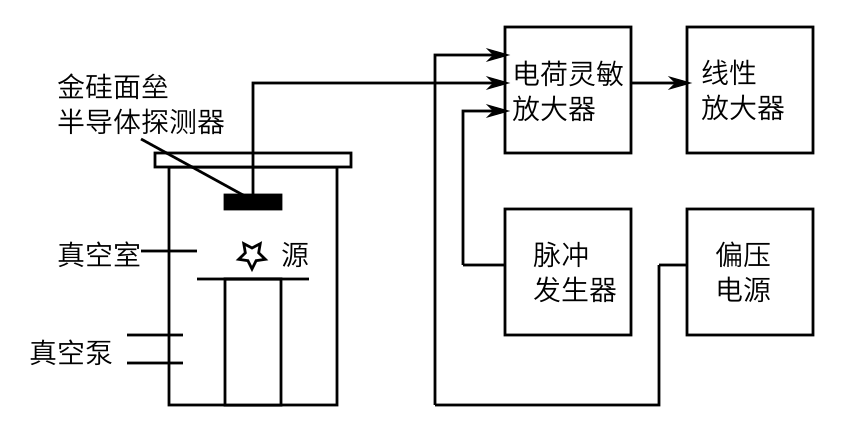
\includegraphics[width=0.4\textwidth]{tu1.png}\\
\xiaowu\song 图~1\begin{minipage}[t]{75mm} \quad 金硅面垒半导体探测器装置示意图。前级电荷放大器的输出信号经过线性放大器放大即可输入至多道等分析仪器进行分析。\\[-1mm]\wuhao
\end{minipage}
\end{center}

但是因为半导体结电容$C_d$的存在,金硅面垒探测器直接输出的脉冲信号幅度是$Q/C_d$,这样就会因为探测器所加偏压的微小变化而造成输出信号的幅度。从而导致探测结果的不精确,所以在探测器后面一般会接上一级前级放大器。在合理的选择前级放大器的电路,放大倍数以及反馈电容后,可以得到放大器输出的电压为
\begin{equation}\label{eq:1}
	V_0 =\frac{Q}{C_f}
\end{equation}
其中$C_f$是反馈电容的大小。具体的等效电路见图2。

\begin{center}
   \def\svgwidth{0.4\textwidth}
   \input{fangdaqi.eps_tex}
\\
\xiaowu\song 图~2\begin{minipage}[t]{75mm} \quad 探测器的等效电路以及前置放大器的电路图。图中$C_d$即为半导体探测器的等效结电容,$C'$为接线电缆等电容,经过前级放大器K倍放大后,若$KC_f>>C_d+C_1$,则最终输出电压满足上述公式\ref{eq:1}中的结果。\\[-1mm]\wuhao
\end{minipage}
\end{center}

通过使用半导体$\alpha$谱仪,我们可以非常方便的得到$\alpha$粒子的能谱,从而能够对$\alpha$粒子与物质的相互作用进行深一步的研究。$\alpha$粒子一般与物质的核外电子发生相互作用,其与电子碰撞使得原子电离,从而损失能量。又因为$\alpha$粒子的质量远远大于电子的质量,因而每次碰撞所转移给电子的能量有一个最大值,同时粒子的方向基本不发生改变。带电粒子在吸收体内单位长度损失的能量被称作线性阻止本领S。将S除以吸收体单位体积内的原子数N,得到物质的阻止截面$\Sigma_e$。 对于$\alpha$离子的阻止截面,可以得到一个经验公式:
\begin{equation}\label{eq:e}
	\Sigma_e=\frac{A_1 EA_2 \{ \frac{A_3}{E/1000}\ln[1+\frac{A_4}{E/1000}+\frac{A_5 E}{E/1000}]\}}{A_1 EA_2+\frac{A_3}{E/1000}\ln[1+\frac{A_4}{E/1000}+\frac{A_5 E}{E/1000}]}
\end{equation}
其中$A_1$到$A_5$是与材料有关的常数。

在知道阻止截面和能量的关系,以及$\alpha$粒子穿过物质后所损失的能量,我们就可以很方便的得到物质的厚度,这也就是通过$\alpha$粒子测量物质厚度方法的原理。
\subsection{实验过程}

\begin{enumerate}
\item 按照图1连接实验装置,并将输出接入多道分析仪。将$\alpha$源$^{239}Pu$放入真空室,抽真空。
\item 调节偏压到180V,通过多道观察输出波形,并通过调整线性放大器使峰位在6V左右。
\item 测量不同偏压下(30V-210V),输出波形的峰位和分辨率随偏压的变化,选择合适的偏压。
\item 在该偏压下测量$\alpha$源的能谱。并将铝吸收膜放入真空室中源和探测器之间,测量能谱峰位的变化。
\item 通过脉冲发生器模拟源并对后续电路进行标定。
\end{enumerate}


\section{实验结果和讨论}
如上述实验过程所述,在准备好实验装置后,调节探测器偏压到180V,通过调整放大器使得$\alpha$的能谱峰位落在了610道处。不同偏压下,探测器探测到的峰位分辨率如下表:

\begin{center}
\bgliu
{\bf 表~1\quad
不同偏压下,探测器探测得到$\alpha$能谱的峰位以及分辨率数据表}\\[0.5mm]
\renewcommand{\arraystretch}{1.5}
\liuhao\song\rm
\newcolumntype{M}{>{\centering\arraybackslash}m{15mm} >{\centering\arraybackslash}m{15mm}
>{\centering\arraybackslash}m{15mm}}
\begin{tabular}{M}
\specialrule{0.1em}{1pt}{1pt}

偏压/V	&	峰位/道	&	分辨率/\%	\\
\midrule
30	&	417	&	9.3	\\
45	&	431	&	8.7	\\
60	&	438	&	8.2	\\
75	&	454	&	7.3	\\
90	&	474	&	6.0	\\
105	&	502	&	5.6	\\
120	&	529	&	5.0	\\
135	&	554	&	4.4	\\
150	&	577	&	4.2	\\
165	&	594	&	3.9	\\
180	&	610	&	3.8	\\
195	&	625	&	3.7	\\
210	&	637	&	3.6	\\
\specialrule{0.1em}{3pt}{2pt}\\[-4mm]
\end{tabular}\\
\renewcommand{\arraystretch}{1.0}
\end{center}
实验中同时观察到$\alpha$能谱从30V偏压下的一个峰位逐渐转变为210V下的两个可分辩的独立的峰位,其中较小的峰位于主峰右侧。具体形状可以参考图5。

做出能谱峰位和分辨率随偏压变化的图如下:

\begin{center}
   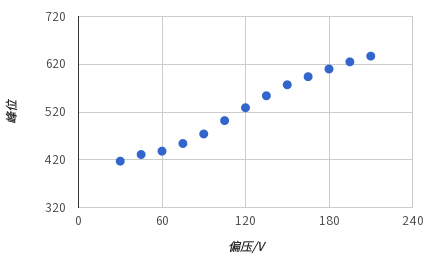
\includegraphics[width=0.4\textwidth]{fengwei.png}
\\
\xiaowu\song 图~3\begin{minipage}[t]{75mm} \quad 探测到的$\alpha$能谱峰位随偏压改变变化图。可以看出偏压越大,峰位也变大并趋于一个稳定的值。\\[-1mm]\wuhao
\end{minipage}
\end{center}

\begin{center}
   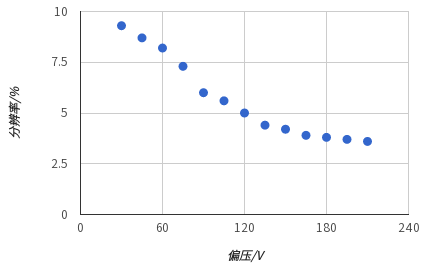
\includegraphics[width=0.4\textwidth]{fenbianlv.png}
\\
\xiaowu\song 图~4\begin{minipage}[t]{75mm} \quad 探测到的$\alpha$能谱峰分辨率随偏压改变变化图。可以看出偏压越大,分辨率越小并且变化幅度也越来越小。\\[-1mm]\wuhao
\end{minipage}
\end{center}

从实验结果可以看出,在我们逐渐增加探测器的反向偏压的时候,探测器探测得到的$\alpha$能谱中峰位也会逐渐变大并趋于一个稳定值,而分辨率也在逐渐变小。对应图谱变化为峰位右移,并且两个峰的区分度变得越来越明显。半导体质谱仪的原理产生了这一现象。半导体的灵敏区厚度和结电容的大小都取决于外加电压,在电压逐渐升高的过程中,灵敏区厚度逐渐变大,从而可以使得$\alpha$沉积的能量变大直至全部被沉积并收集。同时因为探测器的结电容所带来的实际上一个噪声源,随着偏压的升高,结电容逐渐减小,从而改善了探测器的能量分辨率。所以观测得到的现象即为峰位逐渐变大并趋于稳定,而分辨率逐渐变小。但是偏压过高,即可能损坏仪器,同时探测器的漏电流也会增大从而使得分辨率变坏。所以偏压应该选择一个较为合适的范围。在本次测量中,偏压就选择为210V。

选定210V偏压,就可以具体的测量$^{239}Pu$放射源的$\alpha$能谱了。利用多道测量记录得到了图5

\begin{center}
   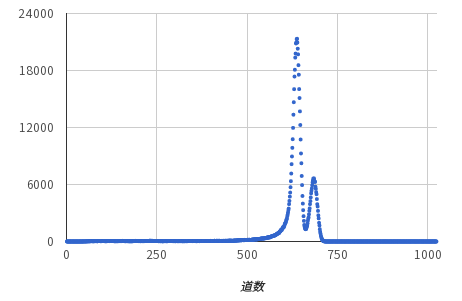
\includegraphics[width=0.4\textwidth]{Pu.png}
\\
\xiaowu\song 图~5\begin{minipage}[t]{75mm} \quad 探测到的$\alpha$能谱图,探测器偏压为210V\\[-1mm]\wuhao
\end{minipage}
\end{center}
可以看出在210V的偏压下,$\alpha$能谱的两个峰是清晰可分辩的。其中较大的峰所处的道数为637道。同样可以分析加入铝膜后的数据。如图6:

\begin{center}
   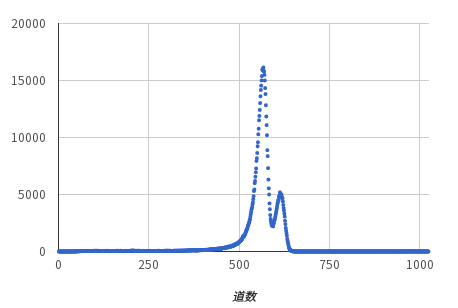
\includegraphics[width=0.4\textwidth]{PuAl.png}
\\
\xiaowu\song 图~6\begin{minipage}[t]{75mm} \quad 探测到的经过铝膜损失能量后的$\alpha$能谱图,探测器偏压为210V\\[-1mm]\wuhao
\end{minipage}
\end{center}
可以看出在经过铝膜之后,$\alpha$粒子自身的能量损失,整体等峰位左移。其主峰峰位为566道。这样就可以计算出经过铝膜以后,$\alpha$粒子损失的能量对应的道数为71道。

随后就是通过脉冲发生器对测量仪器进行标定。首先设定脉冲发生器发生脉冲幅度为5.15V,并通过调整脉冲发生器的校准使其峰位与Pu的峰位重合。即642道为Pu的峰位,同时也是脉冲发生器发生5.15V电压对应的峰位。这样就可以利用脉冲发生器自身的线性来标定测量仪器了。

调节脉冲发生器的幅度,得到以下峰位电压关系。

\begin{center}
\bgliu
{\bf 表~2\quad
脉冲发生器产生不同脉冲幅度时探测器得到的道数关系表。}\\[0.5mm]
\renewcommand{\arraystretch}{1.5}
\liuhao\song\rm
\newcolumntype{M}{>{\centering\arraybackslash}m{22.5mm} >{\centering\arraybackslash}m{22.5mm}
}
\begin{tabular}{M}
\specialrule{0.1em}{1pt}{1pt}

脉冲幅度/V	&	道数	\\
\midrule
5.0	&	619	\\
4.5	&	552	\\
4.0	&	486	\\
3.5	&	419	\\
3.0	&	354	\\
\specialrule{0.1em}{3pt}{2pt}\\[-4mm]
\end{tabular}\\
\renewcommand{\arraystretch}{1.0}
\end{center}
\begin{center}
   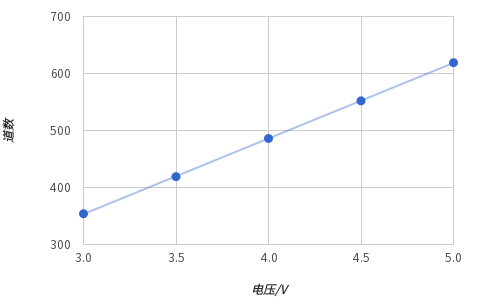
\includegraphics[width=0.4\textwidth]{BD.png}
\\
\xiaowu\song 图~6\begin{minipage}[t]{75mm} \quad 脉冲发生器产生不同脉冲幅度时探测器得到的道数关系图。\\[-1mm]\wuhao
\end{minipage}
\end{center}
通过计算就可以得到道数和脉冲电压的关系为
\begin{equation}
	U = 0.0075X + 0.334
\end{equation}
其中X为道数。又因为$^{239}Pu$衰变$\alpha$粒子的能量为5.15MeV,这样就将能量和道数之间的关系对应起来,从而可以得到经过铝膜后,$\alpha$粒子损失的能量为0.53MeV。

将铝的常数带入公式\ref{eq:2}就可以得到散射截面,从而可以计算得到铝膜的厚度为3.18$\mu m$。


\section{总结和结论}
在本次实验中,随着探测器偏压的增大,探测器探测得到的$^{239}Pu$的$\alpha$粒子峰位逐渐变大,并且分辨率便高。最后选定210V偏压进行测量。

测量得到的$\alpha$能谱图如图5所示,经过铝膜后的能谱图如图6所示,可以看出经过铝膜后$\alpha$粒子的能量降低,通过标定和计算可以得到降低越0.53MeV。进而通过计算可以得到添加的铝膜的厚度为3.18$\mu m$。

\section{致谢}
感谢倪老师的细致讲解以及楼建玲老师为实验做出的准备。
\section{参考文献}

\noindent
[1] Peking Unviersity, Fudan University \ Nuclear Experment
\ Nuclear Publishing House, 1989: 17-23. (in Chinese)

\noindent
 (北京大学,复旦大学.\ 原子核实验\ 原子能出版社,\ 1989: 17-23.)

\end{multicols}

\newpage


\section*{附录:思考题}

14.1 脉冲幅度随偏压增加而增加,并且增加速度逐渐放缓。分辨率随脉冲幅度增加变小,在超过一定值后再增大(本实验中没有观测到)。选择探测器偏压应该在脉冲幅度基本稳定不变时选择分辨率小时的偏压。

14.2 半高宽为0.007V,而幅度为6V,此时分析范围应该约为0-8V,道数应该为2048道左右。此时道宽为0.004V。道数不够或道宽太大时,可以通过偏执放大器将阈值设置为感兴趣范围的下限,放大倍数使得感兴趣区域的上限位于多道的上限,此时就相当于放大感兴趣范围到整个多道范围。

14.3 因为偏压电源影响了电荷放大器,是放大电路的组成部分,关闭偏压就会是的标定不正确。

14.4 如上述实验所说,调整幅度到一个固定值并使用标准校正使得他和$\alpha$源峰值对应以建立脉冲幅度与能量之间的关系,再通过调整脉冲幅度来模拟改变能量从而标定谱仪。

14.5 不放入源,连接探测器和电子学器件,同时利用校准功能外接脉冲发生器模拟产生信号。这样得到的展宽就是电子学噪声以及探测器噪声的展宽

4.1 $\alpha$粒子穿过吸收体之后,本身与吸收体内原子的核外电子碰撞本身就是一个统计过程,所以吸收的能量本身就会有一定的展宽,因而能谱会变宽。

4.2 $\Delta E = [S] \times \Delta x / \sin{\theta}$。 所以能量损失为$1.002\Delta x [S]$以及$1.006\Delta x [S]$

4.3 Am的能量为5485.8keV,$d E = 0.228 \times 19.31 = 4.4 keV$ 所以最后能量为5481.4keV。

4.4 没有测这个膜。。。

4.5 $\alpha$粒子原始的能量为5.15MeV, 铝膜中损失的能量为0.53MeV。取$\delta E = 0.01MeV$,在这个情况下进行叠加,可以得到最后的长度为3.09$\mu m$。

\begin{center}
\bgliu
{\bf 表~3\quad
Al膜厚度计算表。}\\[0.5mm]
\renewcommand{\arraystretch}{1.5}
\liuhao\song\rm
\newcolumntype{M}{>{\centering\arraybackslash}m{18mm} >{\centering\arraybackslash}m{18mm} >{\centering\arraybackslash}m{18mm} >{\centering\arraybackslash}m{18mm}>{\centering\arraybackslash}m{18mm} >{\centering\arraybackslash}m{18mm}
}
\begin{tabular}{M}
\specialrule{0.1em}{1pt}{1pt}

能量/MeV	&	散射截面/$eV\times10^{-15}\times cm^2$	&	行走长度/$\mu m$	&	能量/MeV	&	散射截面	/$eV\times10^{-15}\times cm^2$&	行走长度/$\mu m$	\\
\midrule
5.15	&	27.91	&	0.0595	&	4.88	&	28.96	&	0.0573	\\
5.14	&	27.94	&	0.0594	&	4.87	&	29.00	&	0.0573	\\
5.13	&	27.98	&	0.0593	&	4.86	&	29.04	&	0.0572	\\
5.12	&	28.02	&	0.0593	&	4.85	&	29.08	&	0.0571	\\
5.11	&	28.06	&	0.0592	&	4.84	&	29.12	&	0.0570	\\
5.10	&	28.09	&	0.0591	&	4.83	&	29.17	&	0.0569	\\
5.09	&	28.13	&	0.0590	&	4.82	&	29.21	&	0.0569	\\
5.08	&	28.17	&	0.0589	&	4.81	&	29.25	&	0.0568	\\
5.07	&	28.21	&	0.0589	&	4.80	&	29.29	&	0.0567	\\
5.06	&	28.25	&	0.0588	&	4.79	&	29.33	&	0.0566	\\
5.05	&	28.29	&	0.0587	&	4.78	&	29.37	&	0.0565	\\
5.04	&	28.32	&	0.0586	&	4.77	&	29.42	&	0.0565	\\
5.03	&	28.36	&	0.0585	&	4.76	&	29.46	&	0.0564	\\
5.02	&	28.40	&	0.0585	&	4.75	&	29.50	&	0.0563	\\
5.01	&	28.44	&	0.0584	&	4.74	&	29.54	&	0.0562	\\
5.00	&	28.48	&	0.0583	&	4.73	&	29.59	&	0.0561	\\
4.99	&	28.52	&	0.0582	&	4.72	&	29.63	&	0.0560	\\
4.98	&	28.56	&	0.0581	&	4.71	&	29.67	&	0.0560	\\
4.97	&	28.60	&	0.0581	&	4.70	&	29.72	&	0.0559	\\
4.96	&	28.64	&	0.0580	&	4.69	&	29.76	&	0.0558	\\
4.95	&	28.68	&	0.0579	&	4.68	&	29.80	&	0.0557	\\
4.94	&	28.72	&	0.0578	&	4.67	&	29.85	&	0.0556	\\
4.93	&	28.76	&	0.0577	&	4.66	&	29.89	&	0.0556	\\
4.92	&	28.80	&	0.0577	&	4.65	&	29.93	&	0.0555	\\
4.91	&	28.84	&	0.0576	&	4.64	&	29.98	&	0.0554	\\
4.90	&	28.88	&	0.0575	&	4.63	&	30.02	&	0.0553	\\
4.89	&	28.92	&	0.0574	&	4.62	&	30.07	&	0.0552	\\

\specialrule{0.1em}{3pt}{2pt}\\[-4mm]
\end{tabular}\\
\renewcommand{\arraystretch}{1.0}
\end{center}


\clearpage
%\end{CJK*}
\end{document}

